\section{Theorie}

\subsection{Der Mitführungskoeffizient}

Die Geschwindigkeit des Lichtes in einem ruhenden Medium wird durch die Formel $$v=\frac{c}{n}$$ berechnet, wobei $c = 3\cdot 10^8 m/s$ die Lichgeschwindigkeit im Vakuum und $n$ der Brechungsindex des jeweiligen Mediums ist. Hat das Medium eine Geschwindigkeit w, so ergibt sich folgende Formel für die Geschwindigkeit des Lichtes:
\begin{equation} v = \frac{c}{n} \pm \alpha\cdot w  \end{equation}
$\alpha$ ist hier der Mitführungskoeffizient und es gilt:
\begin{equation} \alpha = 1 - \frac{1}{n^2} - \frac{\lambda\cdot\Delta n}{n \cdot\Delta\lambda} \end{equation}
Fresnel postulierte 1818, dass dieser die Mitführung des Äthers durch die Bewegung des Körpers beschreibt, daher der Name. Er leitete den Wert von $\alpha = 1 - 1/n^2$ her. Nach der experimentellen Widerlegung der Äthertheorie leiteten modernere Theorien, wie die Relativitätstheorie, diesen Faktor genauer her, sodass die oben genannte Formel (2) entstand.

\subsubsection{Herleitung des Mitführungskoeffizienten}

Die Relativitätstheorie besagt, dass wenn ein System $K'$ sich relativ zu einem System $K$ mit der Geschwindigkeit $w$ in x-Richtung bewegt, Orts- und Zeitkoordinaten dieser Systeme durch die Lorentztransformationen zusammenhängen: 

\begin{equation} x' = \gamma (x-wt) \end{equation}
\begin{equation} t' = \gamma \left(t-\frac{wx}{c^2}\right) \end{equation}
\begin{equation} \text{mit \ } \gamma = \frac{1}{\sqrt{1-\frac{w^2}{c^2}}} \end{equation}

Außerdem gilt $y'=y$ und $z'=z$. Aus diesen Formeln ergibt sich die Formel für die relati\-vistische Addition von Geschwindigkeiten:

\begin{equation} v = \frac{v' + w}{1 + \frac{v'\cdot w}{c^2}} \end{equation}

(v und v' sind hier in x-Richtung). Für ein Lichtstrahl der Geschwindigkeit $v' = c/n$ und mit den Näherung $w<<c$ und somit $(1+a)^{-1}\approx 1-a$ und $\frac{w}{c} \approx 0$ erhält man schlussendlich die Fresnelsche Mitführungsformel:

\begin{equation} v\approx \frac{c}{n} \pm \left(1-\frac{1}{n^2}\right)w \end{equation}

Im Fall von der rotierenden Quarzscheibe gilt $w = w_x = w_r = w_i / n$  (siehe hierzu Abbildung 2 in 2.1). Außerdem betrachten wir nun auch die Abhängigkeit des Brechungsindexes eines Mediums von der Frequenz des gebrochenen Lichts, also $n = n(\nu)$. Nämlich folgt aus der Dopplerverschiebung

$$\nu' = \nu\left( 1\mp \frac{w_i}{c}\right)$$

die lineare Näherung für den Brechungsindex

$$n(\nu') = n(\nu) + (\nu' - \nu)\frac{dn}{d\nu} = n(\nu)\left(1 \mp \frac{w_i\cdot\nu}{c\cdot n(\nu)}\frac{dn(\nu)}{d\nu} \right)$$

und somit die Formel für die Geschwindigkeit, nachdem Näherungen ($w_r << c$) gemacht wurden:

\begin{align} 
v & \approx \frac{c}{n} \pm w_r\cdot\left(1 - \frac{1}{n^2} - \frac{w_i}{w_r}\frac{\nu}{n^2}\frac{dn}{d\nu} \right)\\
& = \frac{c}{n} \pm w_r\cdot\left(1 - \frac{1}{n^2} - \frac{w_i}{w_r}\frac{\lambda}{n^2}\frac{dn}{d\lambda} \right)
\end{align}

Bei der Quarzscheibe ergibt sich dann wegen $w_i / w_r = n$ schlussendlich:

\begin{equation}
\boxed{v = \frac{c}{n} \pm \alpha\cdot w = \frac{c}{n} \pm \left(1 - \frac{1}{n^2} - \frac{\lambda}{n}\frac{dn}{d\lambda} \right)w_r}
\end{equation}

Der Term $\frac{\lambda}{n}\frac{dn}{d\lambda}$ wird dabei als Dispersionsterm bezeichnet. Diese Formel verwenden wir, um den theoretischen Wert für $\alpha$ zu berechnen (siehe Aufgabenstellung). Den experimentellen Wert erhalten wir durch die Formel:

\begin{equation} \alpha = \frac{L\cdot\lambda\cdot\Delta\nu}{2\cdot n\cdot\omega\cdot d \cdot x_0} \end{equation}

wobei $L$ die optische Länge des Ringlasers, $d$ die Dicke der Quarzscheibe, $\omega$ die Drehfrequenz der Scheibe und $x_0$ der Auftreffpunkt des Lasers auf die Scheibe.

\subsection{Der Brewsterwinkel}

\begin{figure}[H]
	\centering 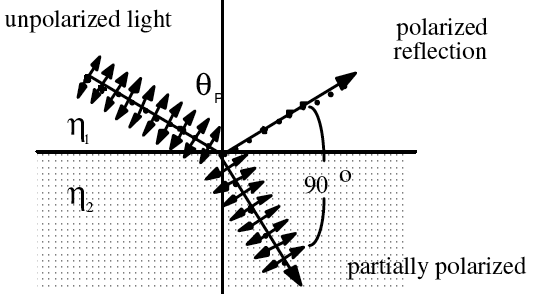
\includegraphics[width = 0.6 \textwidth]{Bilder/brewster.jpg}
	\caption{Zum Brewsterwinkel}
\end{figure}

Der Brewsterwinkel $\theta_B$ ist der Einfallswinkel, für den gilt $\theta_B + \theta' = 90^\circ$, wobei $\theta'$ der Winkel der Brechung ist. Aus den Fresnel-Formeln für Brechung und Reflexion lässt sich berechnen, dass für genau diesen Winkel die reflektierte Welle keine Parallelkomponente hat, d.h. dass die vollständig senkrecht zur Einfallsebene polarisiert ist. Der Winkel lässt sich einfach herleiten:

Aus $$ \frac{\sin(\theta_B)}{\sin(\theta')} = \frac{n_2}{n_1} \text{ \ mit \ } \theta' = 90^\circ - \theta_B$$ folgt sofort die Brewsterbedingung: 
\begin{equation} \tan\theta_B = \frac{n_2}{n_1} \end{equation}

Ist wie in unserem Fall der Strahl linear polarisiert und parallel zur Einfallsebene, so entstehen keine Reflexionsverluste und der Strahl wird komplett durchgelassen.

\subsection{Der He-Ne-Laser}

Ein Helium-Neon-Laser besteht aus einem Glasrohr, in dem sich ein Helium-Neon-Gasgemisch unter Druck befindet. Durch Gasentladung (Energiepumpe) wird das Helium auf den $2^1 S_0$-Zustand angeregt und durch Stöße zweiter Art wird diese Energie auf den $3 s_2$-Zustand eines Neon-Atoms übertragen. An den Enden des Glasrohrs befinden sich Resonatorspiegel, welche vom Neon emittierte Photonen wieder durch das Gasgemisch zurückreflektieren und somit stimulierte Emission induzieren. Diese Resonatorspiegel sind teildurchlässig, so dass ein Teil der Photonen als eigentlicher Laserstrahl herauskommt. Schließlich befinden sich am Laser noch Brewsterfenster, die dafür sorgen, dass nur bestimmt polarisiertes Licht durchkommt.

\begin{figure}[H]
	\centering 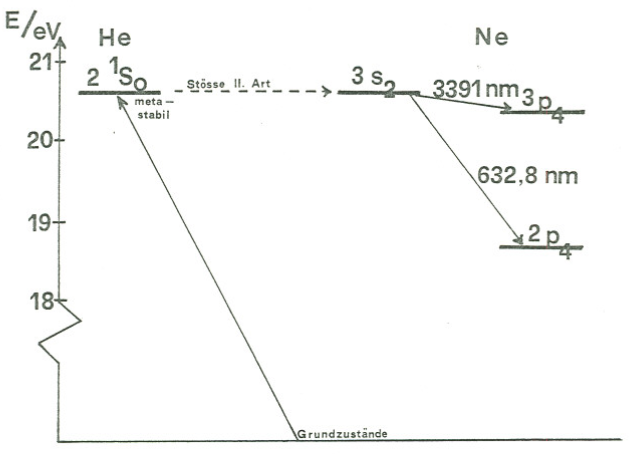
\includegraphics[width = 0.8\textwidth]{Bilder/henelaser.jpg}
	\caption{Termschema des HeNe-Laser}
\end{figure}

\clearpage

























